\documentclass[letterpaper]{article} % DO NOT CHANGE THIS
\usepackage{aaai2027}  % DO NOT CHANGE THIS
\usepackage[hyphens]{url}  % DO NOT CHANGE THIS
\usepackage{graphicx} % DO NOT CHANGE THIS
\urlstyle{rm} % DO NOT CHANGE THIS
\def\UrlFont{\rm}  % DO NOT CHANGE THIS
\usepackage{natbib}  % DO NOT CHANGE THIS AND DO NOT ADD ANY OPTIONS TO IT
\usepackage{caption} % DO NOT CHANGE THIS AND DO NOT ADD ANY OPTIONS TO IT
\frenchspacing  % DO NOT CHANGE THIS
\setlength{\pdfpagewidth}{8.5in} % DO NOT CHANGE THIS
\setlength{\pdfpageheight}{11in} % DO NOT CHANGE THIS

\usepackage{booktabs}
\setcounter{secnumdepth}{2}

\pdfinfo{
/TemplateVersion (2027.1)
}

\title{A Single Fidelity Score Conceals Pathology-Dependent Loss in\\Accelerated Knee MRI}

\author{
    Sachin Mote\textsuperscript{\rm 1},
    Alicem Koyun\textsuperscript{\rm 2},
    Pranjali Changadeo Pingale\textsuperscript{\rm 2}
}
\affiliations{
    \textsuperscript{\rm 1}George Mason University, Fairfax, VA, United States\\
    \textsuperscript{\rm 2}Westcliff University, Irvine, CA, United States\\
    sachinmoteofficial@gmail.com, alicemkoyun@gmail.com, pranjalipingale@gmail.com
}

\begin{document}
\maketitle

\begin{abstract}
Accelerated MRI reconstruction is reported almost universally as a single
whole-image fidelity score, and a growing class of methods now trains without
fully sampled raw data so that it can be deployed where only reconstructed
images exist. We ask whether that score describes what happens to the regions a
radiologist reads. Using the fastMRI knee validation set with fastMRI+ clinical
annotations, we score 218 radiologist-annotated lesion regions from 18 patients
against size-matched control regions drawn from tissue on the same slice. The
answer is that the aggregate is not merely incomplete but unstable. Its sign
depends on the reconstruction: with zero-filling, lesion regions are rendered
\emph{worse} than matched tissue ($-0.024$ SSIM, $p{=}1.9\times10^{-7}$); with
CG-SENSE they are rendered \emph{better} ($+0.038$, $p{=}4.6\times10^{-5}$). Its
sign depends on the metric: for CG-SENSE, SSIM reports $+0.038$ while PSNR
reports $-0.064$\,dB and is indistinguishable from zero ($p{=}0.81$). It also
conceals opposite-signed behaviour across findings --- meniscus tears, 97
regions across 15 patients, are preserved ($+0.055$) while partial-thickness
cartilage defects, 49 regions across 9 patients, are attenuated ($-0.028$) ---
reverses in 7 of 18 patients, and peaks at $R{=}4$ rather than growing with
acceleration. It is, however, insensitive to calibration size across 12, 24 and
48 autocalibration lines, so it is not an artifact of coil-map quality. Because
the reconstruction we measure is the one raw-data-free methods use to
manufacture training targets, a pathology-dependent deficit in it propagates
into every model trained against it. We release the protocol, splits and code.
\end{abstract}

\noindent\textbf{Code ---} \url{https://github.com/sachinmoteofficial/AAAI27}

\section{Introduction}

A patient scanned on an accelerated protocol is scanned for a reason: someone is
looking for a finding. Yet the reconstruction that produces their images is
evaluated, in nearly every paper, by a whole-image distortion score computed
against a fully sampled reference \citep{zbontar2018fastmri}. That score weights
every pixel equally --- cortical bone, marrow, muscle, background air, and the
few hundred pixels that contain the finding. It is a reasonable engineering
summary. It is not obviously a clinical one.

The gap matters more as reconstruction moves toward the settings that motivate
health-intelligence research. A recent line of work trains physics-driven
reconstruction networks without any fully sampled raw data, using only routine
reconstructed images, so that hospitals which never receive raw $k$-space can
still benefit from accelerated imaging \citep{alcalar2025cupid}. The stated
motivation is equity of access. The training target in that setting is a
parallel-imaging reconstruction of the undersampled acquisition. If that target
is itself selectively degraded where pathology lives, every model trained toward
it inherits the deficit, and a whole-image score will not reveal it.

We test that premise directly rather than arguing it. The fastMRI+ annotations
\citep{zhao2021fastmriplus} provide radiologist-drawn bounding boxes for
clinical findings on fastMRI knee slices, which makes it possible to score a
reconstruction where a reader would look, and to compare that against matched
tissue elsewhere in the same image. What we find is stronger than incompleteness:
the aggregate's sign is not a property of the data alone but of the
reconstruction and the metric chosen to summarise it.

\paragraph{Contributions.}
\begin{itemize}
\item A region-controlled evaluation protocol in which each annotated lesion is
      compared against size-matched controls from the same slice, holding
      patient, slice, coil configuration and region size fixed.
\item The finding that the lesion-versus-tissue comparison \emph{reverses sign}
      between two standard reconstructions of the same data, and again between
      two standard metrics of the same reconstruction.
\item Evidence of opposite-signed behaviour across finding types, reported with
      patient counts so that single-patient labels are not mistaken for effects.
\item Robustness analyses over acceleration, calibration size, region size and
      patient, and released splits, protocol and code.
\end{itemize}

\paragraph{Scope.} This is a measurement study. We propose no reconstruction
method and make no claim about diagnostic accuracy: SSIM inside a bounding box
is a fidelity proxy, not a detection endpoint. What we claim is that the summary
statistic the field reports does not describe the regions clinicians read, and
that its instability is measurable. Figure~\ref{fig:overview} summarises the
protocol, the result and the controls.


\begin{figure}[t]
\centering
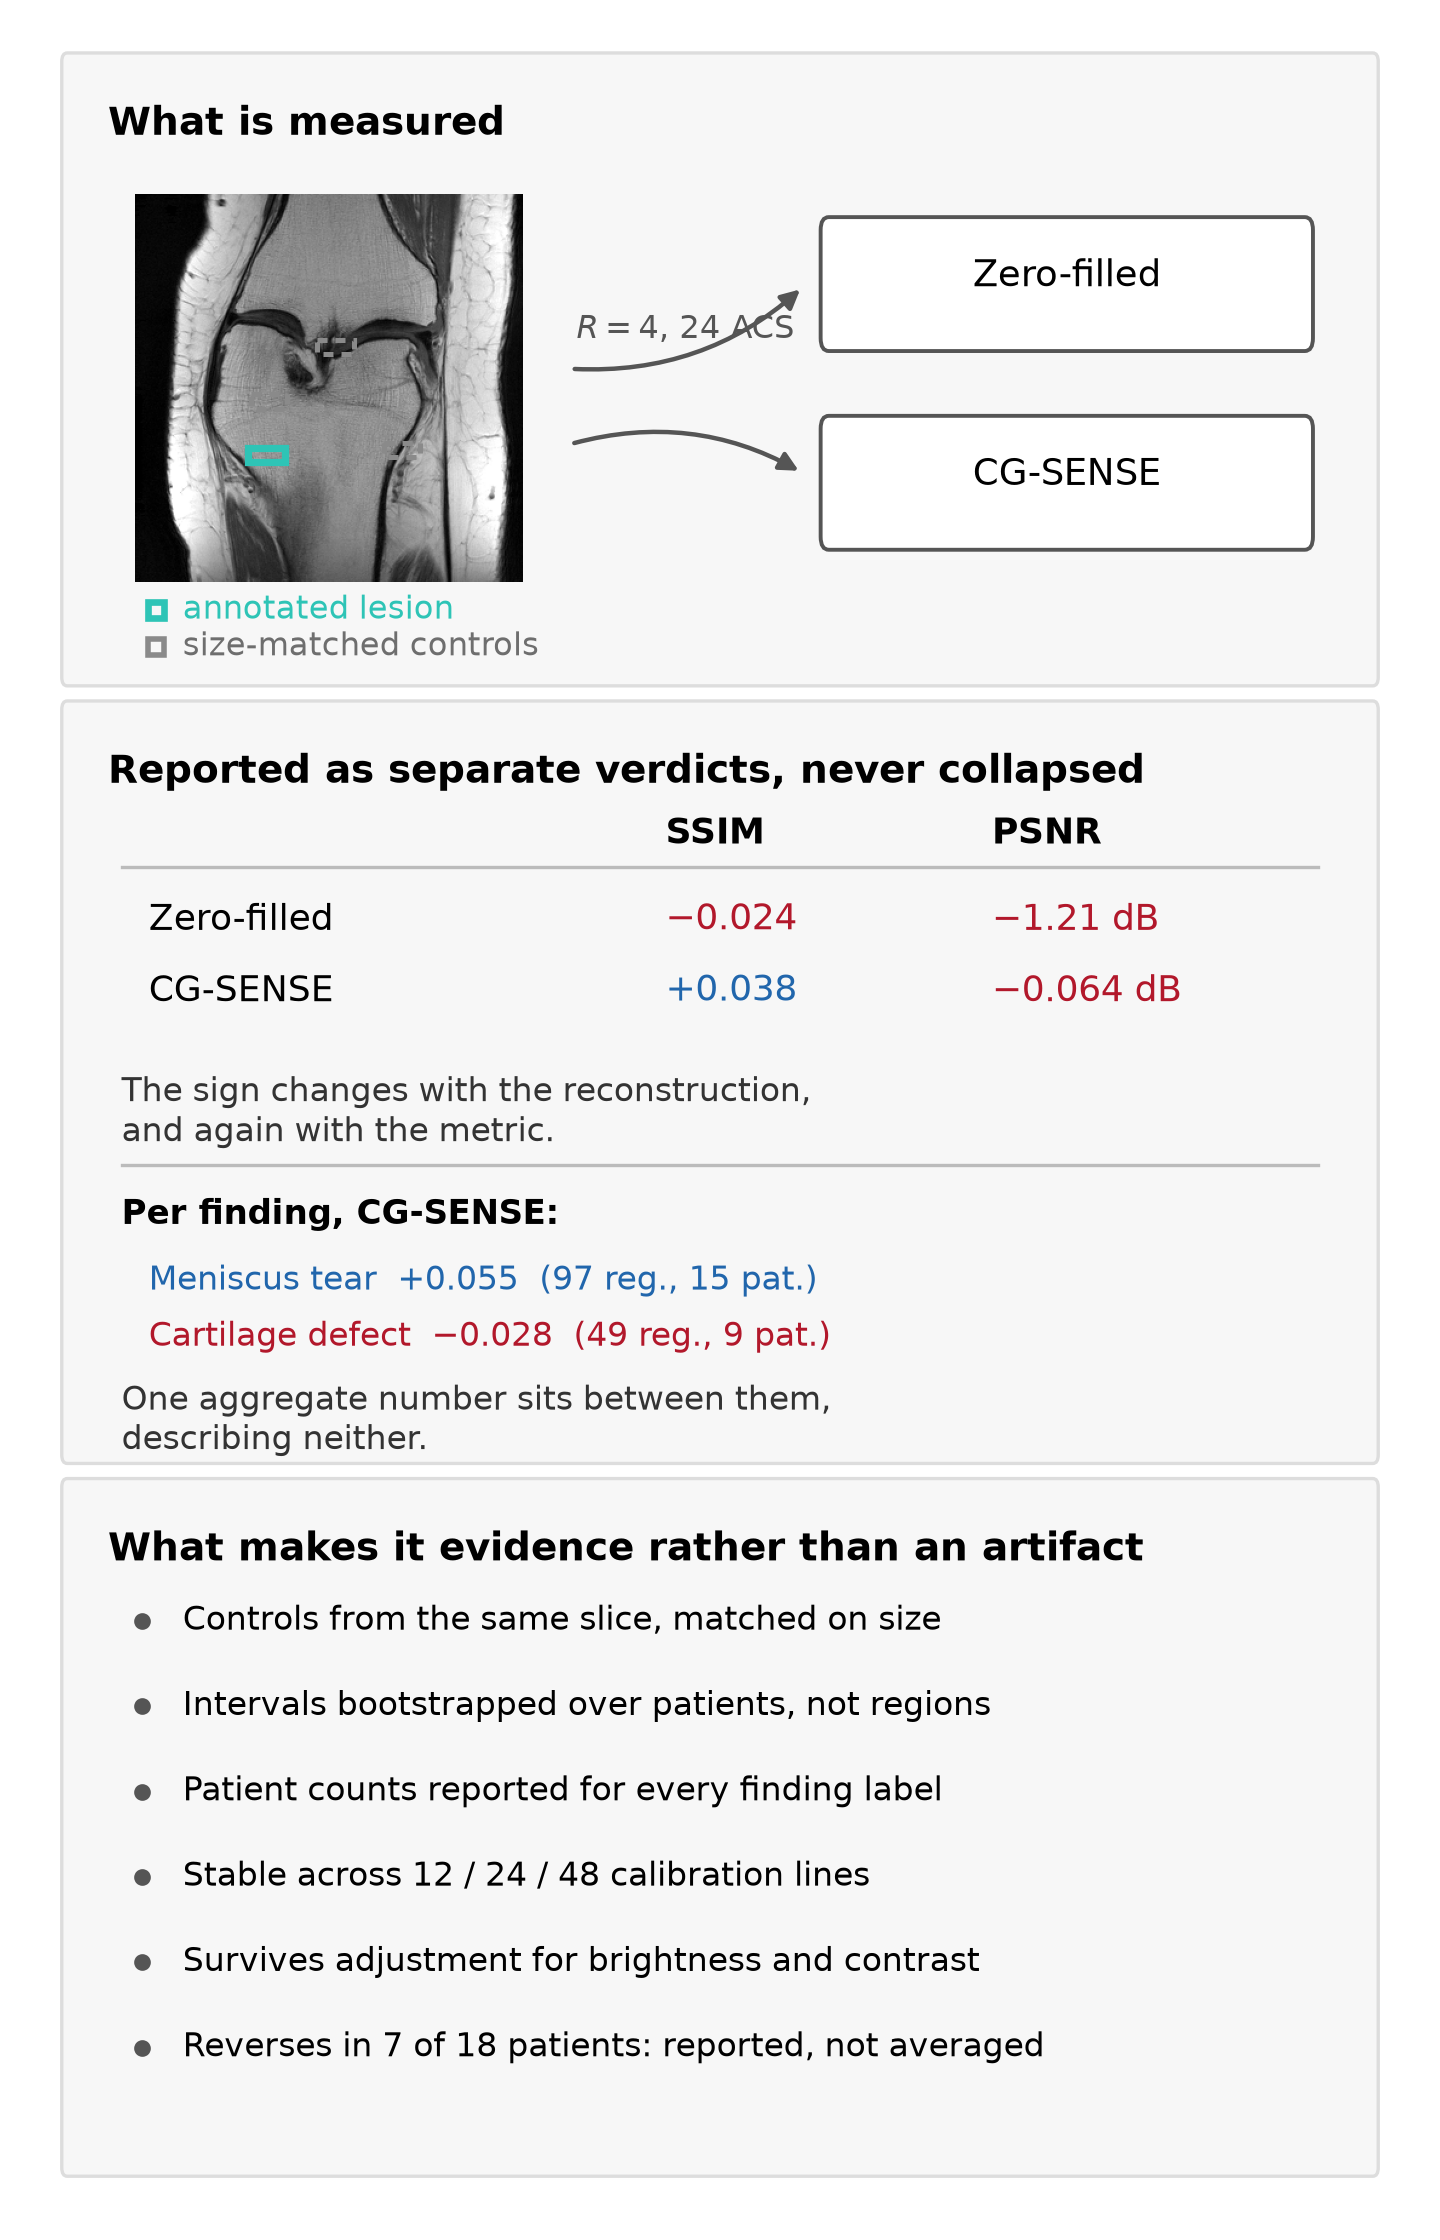
\includegraphics[width=\columnwidth]{figures/fig0_overview.png}
\caption{\textbf{Protocol overview.} \emph{Top:} each annotated lesion region is
compared against size-matched control regions drawn from tissue on the same
slice, and the same measurements are reconstructed two ways at $R{=}4$ with 24
autocalibration lines. \emph{Middle:} the lesion-versus-tissue difference
changes sign between the two reconstructions, and again between the two metrics
most often reported together; decomposed by finding, the two adequately-sampled
labels also disagree in sign, so a single aggregate sits between them.
\emph{Bottom:} the design choices that make the comparison evidence rather than
an artifact of region appearance, calibration or averaging.}
\label{fig:overview}
\end{figure}

\section{Related Work}

\paragraph{Parallel imaging and accelerated reconstruction.}
Modern accelerated MRI rests on parallel imaging --- SENSE
\citep{pruessmann1999sense} in the image domain and GRAPPA
\citep{griswold2002grappa} in $k$-space --- later combined with sparsity priors
\citep{lustig2007sparse} and, more recently, with learned unrolled networks
\citep{hammernik2018variational}. Coil sensitivity estimation from a small
autocalibration region, which our protocol also performs, is standard practice
\citep{uecker2014espirit}. We use CG-SENSE as the object of measurement because
it is the reconstruction that raw-data-free training uses as its target, not
because it is state of the art.

\paragraph{How reconstruction is evaluated.}
The fastMRI benchmark \citep{zbontar2018fastmri} established PSNR and SSIM
\citep{wang2004ssim} against a fully sampled reference as the standard currency,
and the 2020 challenge \citep{muckley2021results} documented that these metrics
can rank methods differently from radiologist assessment. Practice has
nonetheless kept the scalar as the headline number, typically a single mean over
a test split without stratification by anatomy or finding. Our results give a
concrete mechanism for the divergence that challenge observed: the two metrics
do not merely differ in magnitude, they disagree in sign on the subregions that
carry the diagnosis.

\paragraph{Pathology-aware evaluation.}
fastMRI+ \citep{zhao2021fastmriplus} supplied the clinical annotations that make
lesion-level scoring possible: bounding boxes with a disease label, drawn per
slice. Recent work evaluates pathology preservation for models trained
\emph{with} raw data, and studies how clinically relevant detail varies across
candidate reconstructions. Our contribution is complementary and deliberately
narrower, and differs methodologically in comparing each lesion against
size-matched controls from the same slice rather than against a whole-image
average.

\paragraph{Training without raw data.}
Self-supervised reconstruction learns from undersampled acquisitions alone
\citep{yaman2020ssdu}. CUPID \citep{alcalar2025cupid} goes further and trains
from routine reconstructed images using a parallel-imaging fidelity term and a
compressibility term, explicitly targeting sites without raw-data access; its
reported evidence is whole-image quality. Related work introduces designed
perturbations and sparse-domain consistency \citep{alcalar2025spic}. In both,
the quality of the surrogate target is load-bearing, which is what makes
measuring it worthwhile.

\section{Method}

\subsection{Data and Cohort}
We use the fastMRI multi-coil knee validation set, restricted to the
\texttt{CORPD\_FBK} acquisition (coronal proton density without fat
suppression), which contains 100 volumes. We retain the 49 volumes with 368
phase-encode lines so that matrix size is constant across the cohort, avoiding
any need to crop or pad $k$-space. We then draw a subject-wise split: 15
patients for training (unused here; released for the follow-up study) and 19 for
test, every test patient carrying at least one fastMRI+ annotation. From each
test patient we take the central 20 slices, giving 380 test slices, of which 141
carry at least one annotated finding and contribute 218 annotated regions. The
central band is a choice rather than an inherited convention; the released code
exposes it as a parameter.

\subsection{Preprocessing}
fastMRI knee $k$-space is twofold oversampled along readout. We remove the
oversampling in the image domain --- inverse Fourier transform along readout,
centre-crop $640 \rightarrow 320$, transform back --- giving $320\times368$
images with 15 coils. Coil sensitivity maps are estimated from the 24 central
autocalibration lines: the ACS block is Hann-windowed along phase encode,
inverse Fourier transformed per coil, and divided by the root-sum-of-squares
across coils, with values below 2\% of the maximum set to zero. We validated the
maps by comparing the coil-combined fully sampled image against the
\texttt{reconstruction\_rss} volume stored in each source file: correlation
$0.999$, NRMSE $0.062$. The residual difference is expected, since a
SENSE-combined image and a root-sum-of-squares image differ by construction in
low-signal regions. We use ACS-derived maps rather than ESPIRiT so the pipeline
has no dependency outside NumPy and SciPy; absolute values therefore will not
match published tables, but every comparison reported here is internal and
paired.

\subsection{Undersampling and Reconstruction}
We use an equidistant phase-encode mask with acceleration $R$ and a central
autocalibration block, with phase-encode lines carrying no signal marked as
known. The realised sampled fraction is consequently higher than $1/R$ ---
$0.582$, $0.372$ and $0.266$ at $R{=}2,4,8$ --- a property of the mask
convention we inherit rather than an error. We reconstruct two ways: zero-filled
(the adjoint $E^{H}y$) and CG-SENSE, 30 conjugate-gradient iterations on
$E^{H}E x = E^{H} y$ without regularisation. The latter is the identical
operator and iteration count that CUPID uses to construct its clinical-image
surrogate.

\subsection{Region Protocol}
For every annotated slice we compute an SSIM map against the fully sampled
coil-combined reference, using a Gaussian window with $\sigma{=}1.5$ and the
reference maximum as dynamic range. For each fastMRI+ box we record mean SSIM
and PSNR inside the box. We then draw five control regions of \emph{identical}
size from the same slice, each required to lie entirely within eroded tissue and
to be disjoint from every annotated box on that slice, and record the same
statistics. The reported quantity is the paired difference, lesion minus the
mean of its controls. This pairing is what distinguishes the measurement from a
whole-image comparison: region size, slice, patient and coil configuration are
held fixed, so the only varying factor is whether the region contains an
annotated finding.

\subsection{Statistics}
Differences are tested with a two-sided Wilcoxon signed-rank test over regions.
Confidence intervals are subject-clustered bootstrap percentile intervals (5000
resamples over the patients contributing regions), the appropriate unit of
resampling because regions within a patient are correlated. For every label we
report both the number of regions and the number of \emph{patients} those
regions come from, because several labels concentrate in one or two knees and a
region count alone would overstate the evidence.

\section{Results}

\subsection{The Whole-Image Comparison Is Null}
Before the controlled analysis we ran the comparison the literature implies:
whole-image SSIM against in-box SSIM. For CG-SENSE at $R{=}4$ it is null ---
global $0.694$ versus in-box $0.702$, difference $-0.008$, 95\% CI
$[-0.036,+0.016]$, $p{=}0.38$, with lesion regions worse on 46.8\% of slices.
For zero-filled reconstruction the same comparison is significant but tiny in
the opposite direction ($+0.014$, $p{=}0.001$). We report this because it is the
comparison a reader expects, and because it is confounded: a whole-image average
includes background air, where SSIM behaves differently than in textured tissue,
while lesion boxes sit in the anatomical interior. The controlled comparison
replaces it.

\subsection{The Comparison Reverses Between Reconstructions}
Table~\ref{tab:arms} gives the central result. Under zero-filling, lesion
regions are rendered \emph{worse} than size-matched tissue on the same slice:
$-0.024$ SSIM (95\% CI $[-0.036,-0.013]$, $p{=}1.9\times10^{-7}$) and
$-1.21$\,dB PSNR ($p{=}4.0\times10^{-6}$). Under CG-SENSE, reconstructed from
exactly the same measurements with the same mask and the same coil maps, the
comparison inverts: $+0.038$ SSIM (95\% CI $[+0.005,+0.070]$,
$p{=}4.6\times10^{-5}$).

The inversion is not a quirk of the aggregate. For meniscus tears --- the
best-sampled label, 97 regions across 15 patients --- the difference moves from
$-0.031$ under zero-filling to $+0.055$ under CG-SENSE. For partial-thickness
cartilage defects (49 regions, 9 patients) it stays negative, $-0.012$ to
$-0.028$. A reader told only that a method ``achieves SSIM $0.73$'' learns
nothing about which of these regimes they are in.

\begin{table}[t]
\centering
\small
\begin{tabular}{llrrr}
\toprule
Reconstruction & Metric & lesion & control & $\Delta$ \\
\midrule
Zero-filled & SSIM & 0.732 & 0.757 & $-0.024$$^{*}$ \\
 & PSNR & 28.486 & 29.697 & $-1.211$\,dB$^{*}$ \\
CG-SENSE & SSIM & 0.688 & 0.651 & $+0.038$$^{*}$ \\
 & PSNR & 28.589 & 28.653 & $-0.064$\,dB \\
\bottomrule
\end{tabular}
\caption{\textbf{The comparison reverses between reconstructions and between
metrics.} Lesion regions versus size-matched tissue controls on the same slice,
$R{=}4$, 24 ACS lines, 218 regions from 18 patients. $^{*}$ marks $p<0.05$
(two-sided Wilcoxon signed-rank over regions). Zero-filling renders lesions
worse than tissue on both metrics; CG-SENSE renders them better on SSIM and
indistinguishable on PSNR.}
\label{tab:arms}
\end{table}

\subsection{The Two Standard Metrics Disagree in Sign}
Within the CG-SENSE arm, SSIM reports $+0.038$ in favour of lesion regions while
PSNR reports $-0.064$\,dB against them, with a confidence interval spanning zero
($p{=}0.81$). The two metrics most commonly reported side by side in
reconstruction papers therefore do not merely differ in sensitivity here; they
point in opposite directions on the regions that carry the diagnosis. Under
zero-filling they agree, both negative. Whatever the aggregate number is
measuring, it is not a stable property of the reconstruction's clinical
fidelity.

\subsection{The Aggregate Averages Over Opposite Signs}
Table~\ref{tab:perlabel} and Figure~\ref{fig:perlabel} decompose the CG-SENSE
arm by finding. Two labels carry enough patients to support an estimate.
Meniscus tears (97 regions, 15 patients) are reconstructed $+0.055$ better than
matched tissue; partial-thickness cartilage defects (49 regions, 9 patients)
$-0.028$ worse. These point in opposite directions and the aggregate sits
between them, describing neither.

The remaining labels are reported for completeness but must not be read as
effects. Low-grade ACL sprain ($-0.219$) and patellar retinaculum sprain
($+0.209$) each come from a \emph{single} patient, so their subject-clustered
intervals are degenerate and are omitted. Joint effusion ($+0.150$) and
high-grade ACL sprain ($-0.015$) come from two patients each. These are
observations about individual knees, not population estimates, and we mark them
rather than drop them.

\begin{table}[t]
\centering
\small
\begin{tabular}{lrrrrr}
\toprule
Finding & $n$ & subj. & $\Delta$SSIM & 95\% CI & adj. \\
\midrule
ACL sprain, low grade & 7 & 1 & $-0.219$ & --- & $-0.165$ \\
Cartilage, partial-thickness defect & 49 & 9 & $-0.028$ & $[-0.091,+0.036]$ & $-0.031$ \\
ACL sprain, high grade & 21 & 2 & $-0.015$ & $[-0.018,-0.013]$ & $+0.008$ \\
Meniscus tear & 97 & 15 & $+0.055$ & $[-0.002,+0.098]$ & $+0.017$ \\
Joint effusion & 21 & 2 & $+0.150$ & $[+0.143,+0.158]$ & $+0.092$ \\
MCL sprain, low--moderate & 11 & 5 & $+0.170$ & $[+0.074,+0.218]$ & $+0.065$ \\
Patellar retinaculum, high grade & 6 & 1 & $+0.209$ & --- & $+0.107$ \\
\midrule
All regions & 218 & 18 & $+0.038$ & $[+0.006,+0.070]$ & --- \\
\bottomrule
\end{tabular}
\caption{\textbf{Per-finding fidelity at $R{=}4$ under CG-SENSE.} $n$ is
regions; \emph{subj.} is distinct patients. Intervals are subject-clustered
bootstrap percentiles, omitted where one patient contributes every region.
\emph{adj.} is the effect after adjusting for region brightness, variance,
contrast and gradient energy. Only meniscus tear and cartilage defect rest on
more than five patients.}
\label{tab:perlabel}
\end{table}

\begin{figure}[t]
\centering
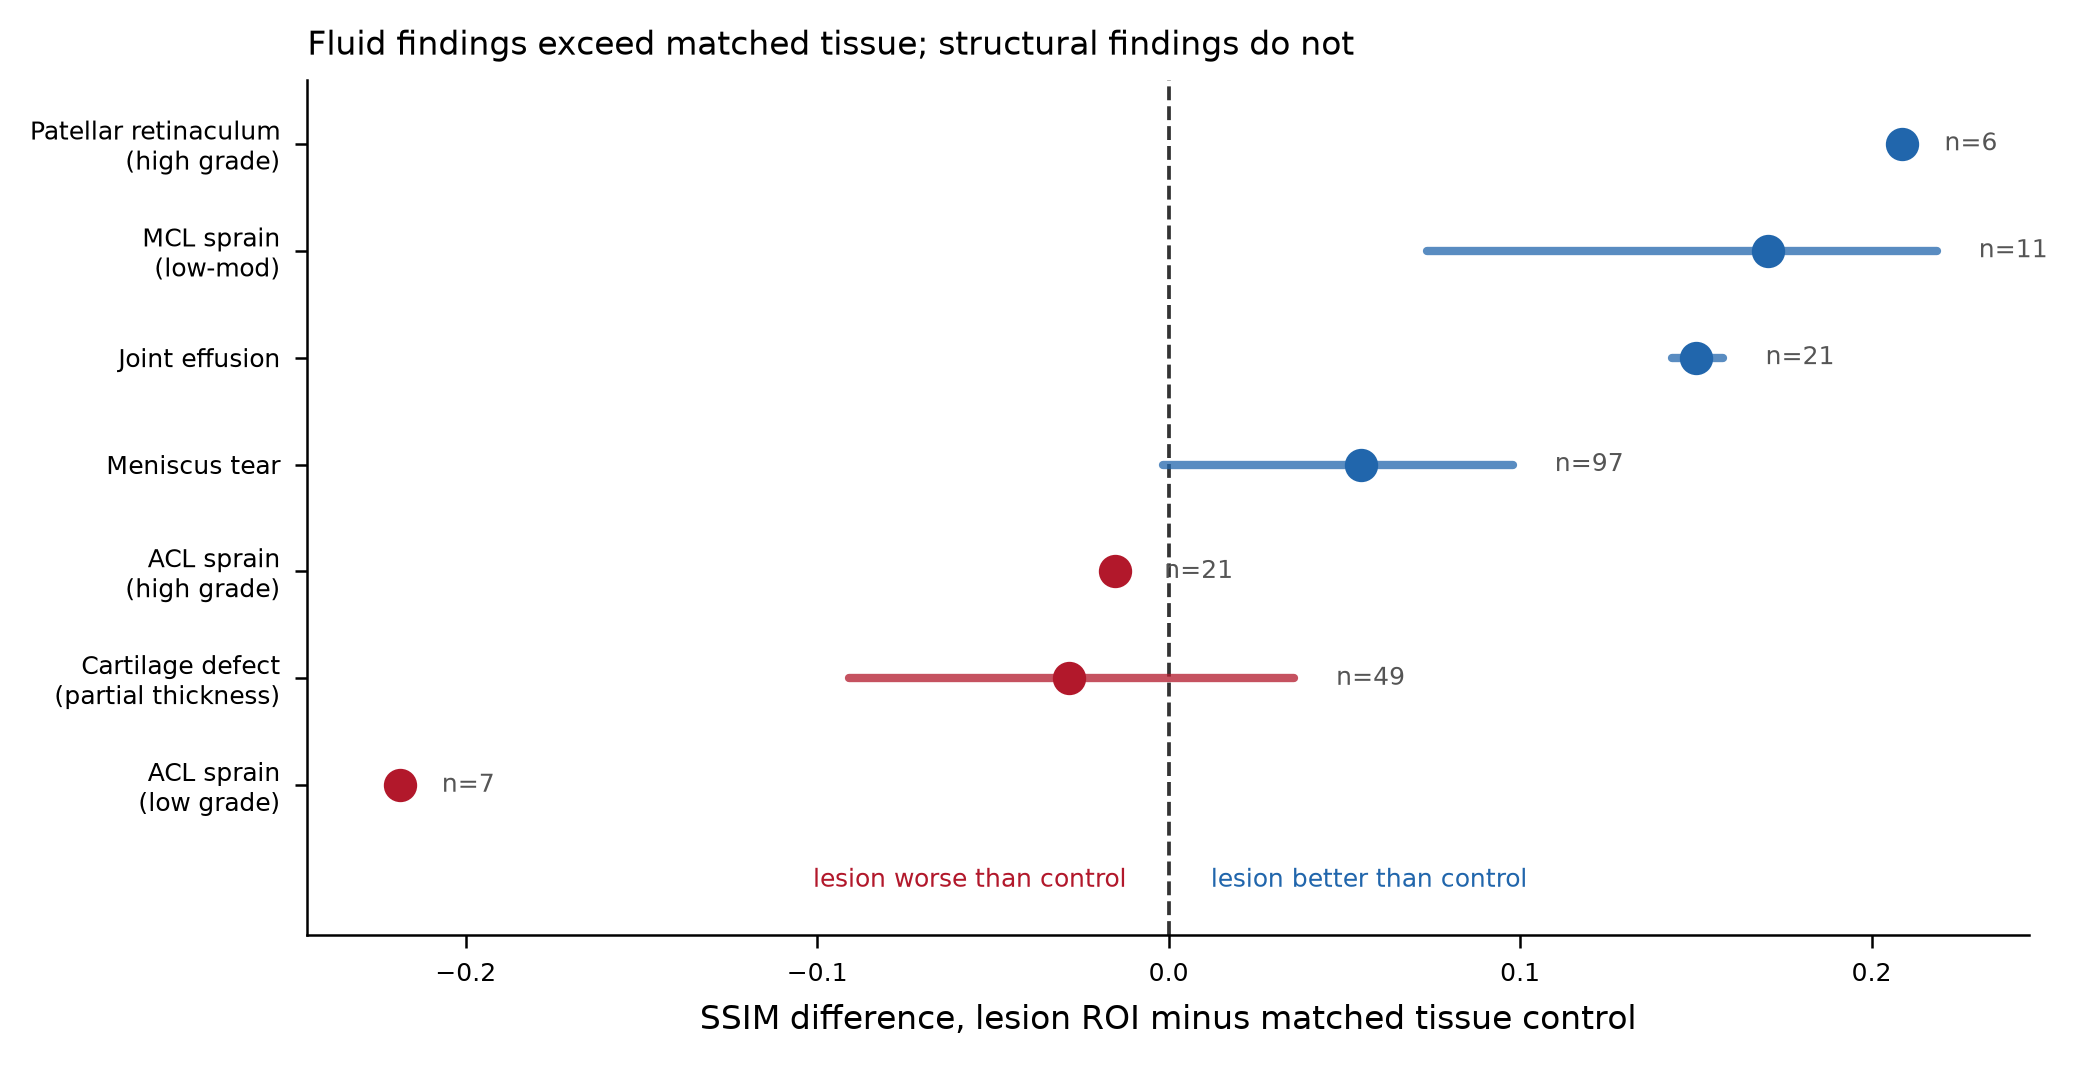
\includegraphics[width=\columnwidth]{figures/fig1_per_label.png}
\caption{\textbf{Per-label fidelity difference at $R{=}4$}, lesion region minus
size-matched tissue control, with subject-clustered bootstrap 95\% intervals.
Positive means the lesion is reconstructed more faithfully than surrounding
tissue. See Table~\ref{tab:perlabel} for the patient counts that qualify these
estimates.}
\label{fig:perlabel}
\end{figure}

\subsection{It Is Not a Region-Appearance Artifact}
SSIM runs high in bright, homogeneous regions, so the positive effects invite
the objection that the metric, not the reconstruction, produces the split. The
data contradict the premise: lesion regions are \emph{darker} than their
controls (normalised mean $0.275$ versus $0.341$, $p{=}4.0\times10^{-14}$) and
\emph{higher} in contrast ($0.665$ versus $0.493$, $p{=}2.9\times10^{-16}$),
with higher variance and gradient energy. Regressing the paired difference on
label indicators together with lesion-minus-control differences in mean,
variance, contrast and gradient energy leaves the pattern intact: cartilage
defects move from $-0.028$ to $-0.031$ and meniscus tears from $+0.055$ to
$+0.017$. Adjustment shrinks the positive effects and leaves the negative one,
the direction consistent with a real structural effect.

\subsection{It Is Not a Calibration Artifact}
A second objection is that our ACS-derived coil maps are too coarse, and that
better calibration would remove the effect. Table~\ref{tab:acs} repeats the
CG-SENSE measurement with 12, 24 and 48 autocalibration lines. The aggregate
moves from $+0.0339$ to $+0.0375$ to $+0.0369$, and the structural and fluid
groups are stable to within $0.006$ across a fourfold change in calibration
data. Whatever drives the split, it is not the quality of the coil maps.

\begin{table}[t]
\centering
\small
\begin{tabular}{lrrr}
\toprule
ACS lines & all regions & structural & fluid \\
\midrule
12 & $+0.0339$ & $-0.0474$ & $+0.0783$ \\
24 & $+0.0375$ & $-0.0421$ & $+0.0810$ \\
48 & $+0.0369$ & $-0.0422$ & $+0.0801$ \\
\bottomrule
\end{tabular}
\caption{\textbf{The effect is insensitive to calibration size.} CG-SENSE at
$R{=}4$ with 12, 24 and 48 autocalibration lines. Structural findings are
cartilage defects and ACL sprains; fluid findings are the remainder. A fourfold
change in calibration data moves the aggregate by $0.004$.}
\label{tab:acs}
\end{table}

\subsection{It Reverses Across Patients and Varies With Region Size}
Averaged within patient, the CG-SENSE difference is negative in 7 of 18 patients
and ranges from $-0.144$ to $+0.238$. The aggregate is therefore a population
mean over patients who differ in sign, not a uniform phenomenon. For the
deployment question --- will this reconstruction preserve findings in
\emph{this} patient --- that heterogeneity is the relevant quantity and is
invisible in any single scalar. Stratified by region area
(Table~\ref{tab:size}), small regions show $+0.036$, medium $+0.002$ and large
$+0.075$; the middle stratum is indistinguishable from zero. Large annotated
regions are dominated by effusions and bulk findings, so size and finding type
are partially confounded and we report the stratification without interpreting
it as an independent size effect.

\begin{table}[t]
\centering
\small
\begin{tabular}{lrrrr}
\toprule
Region size & $n$ & median area & $\Delta$SSIM & $p$ \\
\midrule
Small & 73 & 216\,px & $+0.036$ & 0.012 \\
Medium & 72 & 501\,px & $+0.002$ & 0.978 \\
Large & 73 & 1328\,px & $+0.075$ & 0.000 \\
\bottomrule
\end{tabular}
\caption{\textbf{Fidelity difference by region area} (tertiles), CG-SENSE at
$R{=}4$. $p$ is a two-sided Wilcoxon signed-rank test within the stratum. Region
size and finding type are partially confounded.}
\label{tab:size}
\end{table}

\subsection{The Effect Is Not Monotone in Acceleration}
Table~\ref{tab:accel} and Figure~\ref{fig:accel} sweep $R \in \{2,4,8\}$.
Grouping labels by the sign of their $R{=}4$ effect, the structural group runs
$+0.003$, $-0.042$, $-0.002$ and the fluid group $+0.012$, $+0.081$, $+0.039$.
The deficit for structural findings appears at $R{=}4$ and compresses again at
$R{=}8$. We read this as saturation --- by $R{=}8$ enough fidelity is lost
everywhere that the contrast between lesion and control narrows --- but we did
not test that mechanism and report the non-monotonicity as an observation. It
matters practically: a study measuring only $R{=}8$ would have concluded there
was nothing to see.

\begin{table}[t]
\centering
\small
\begin{tabular}{lrrr}
\toprule
& $R{=}2$ & $R{=}4$ & $R{=}8$ \\
\midrule
Sampled fraction & 0.582 & 0.372 & 0.266 \\
All regions & $+0.009$ & $+0.038$ & $+0.024$ \\
 \quad 95\% CI & \small$[+0.00,+0.02]$ & \small$[+0.01,+0.07]$ & \small$[-0.00,+0.04]$ \\
Structural findings & $+0.003$ & $-0.042$ & $-0.002$ \\
 \quad 95\% CI & \small$[-0.00,+0.01]$ & \small$[-0.08,+0.00]$ & \small$[-0.03,+0.01]$ \\
Fluid / bulk findings & $+0.012$ & $+0.081$ & $+0.039$ \\
 \quad 95\% CI & \small$[+0.01,+0.02]$ & \small$[+0.04,+0.12]$ & \small$[+0.01,+0.07]$ \\
\bottomrule
\end{tabular}
\caption{\textbf{Fidelity difference against acceleration.} The sampled fraction
exceeds $1/R$ because autocalibration and signal-free phase-encode lines are
counted as acquired. Groups are defined by the sign of the $R{=}4$ per-label
effect.}
\label{tab:accel}
\end{table}

\begin{figure}[t]
\centering
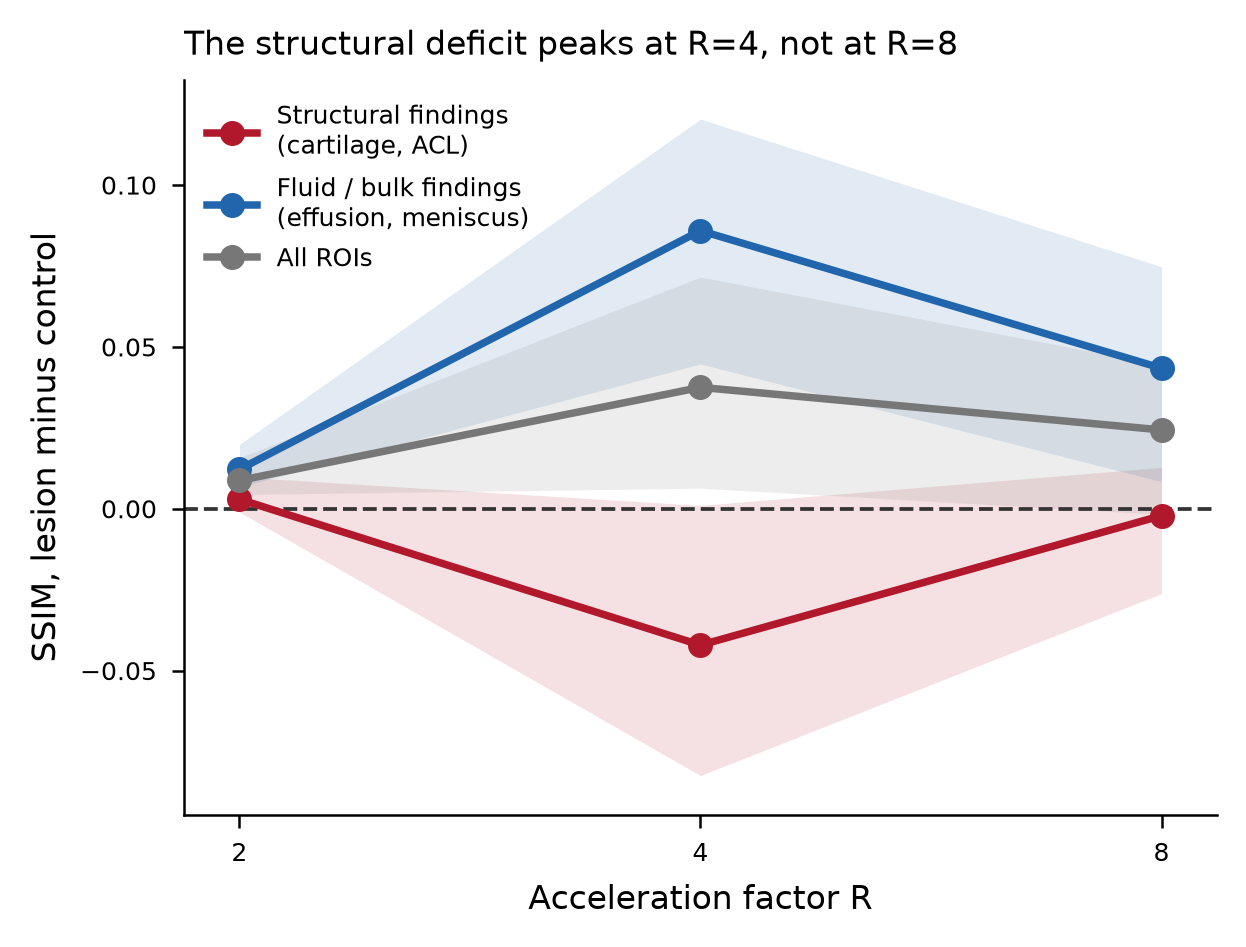
\includegraphics[width=\columnwidth]{figures/fig2_acceleration.png}
\caption{\textbf{Fidelity difference against acceleration}, grouped by the sign
of the $R{=}4$ per-label effect. Bands are subject-clustered bootstrap 95\%
intervals. The structural deficit is largest at $R{=}4$ and compresses at
$R{=}8$.}
\label{fig:accel}
\end{figure}

\begin{figure*}[t]
\centering
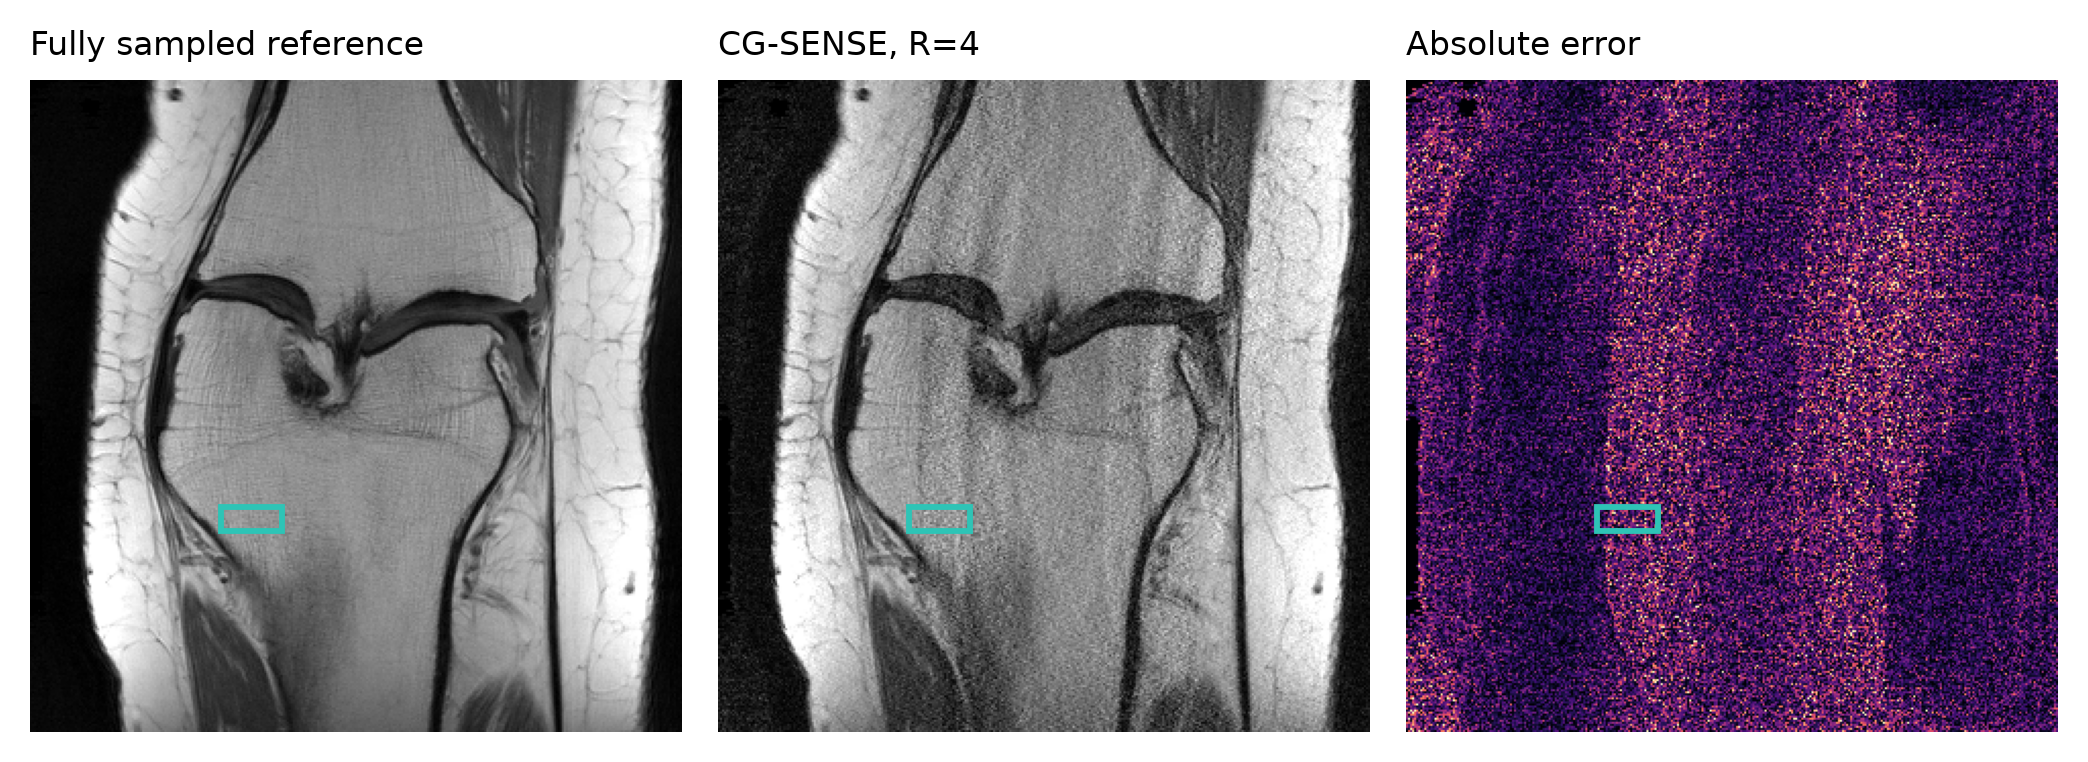
\includegraphics[width=0.92\textwidth]{figures/fig3_example.png}
\caption{\textbf{A representative slice.} \emph{Left:} fully sampled
coil-combined reference. \emph{Centre:} CG-SENSE at $R{=}4$ with 24 ACS lines.
\emph{Right:} absolute error. The teal box marks an annotated partial-thickness
cartilage defect, one of the regions where fidelity falls below matched tissue
on the same slice. Error is not uniformly distributed over the field of view,
which is the premise a whole-image average discards.}
\label{fig:example}
\end{figure*}

\section{Discussion and Limitations}

The practical reading is narrow and we state it narrowly. A single whole-image
fidelity number, reported as the summary of a reconstruction method, is
compatible with opposite-signed behaviour across finding types, across patients,
and --- most awkwardly --- across the reconstruction and the metric used to
produce the number. The same 218 regions yield $-0.024$ or $+0.038$ depending on
which of two standard reconstructions is applied, and $+0.038$ or $-0.064$\,dB
depending on which of two standard metrics is reported. Reporting fidelity
stratified by finding type, with patient counts attached, costs nothing once
annotations exist.

\paragraph{Implication for training without raw data.}
The reconstruction we measured is not an arbitrary baseline; it is the object
that raw-data-free methods treat as ground truth. If the surrogate target
attenuates a class of findings, a network trained to match it is being taught
that the attenuated version is correct, and no quantity of training data repairs
a systematically biased target. Whether a trained reconstruction inherits,
amplifies or corrects the split we measure is an empirical question our released
splits and preprocessing are built to answer, and that we have not answered.

\paragraph{Limitations.}
First and most important, sample size at the label level: only meniscus tear and
partial-thickness cartilage defect rest on more than five patients, and two
labels rest on one patient each. We report patient counts precisely so those
rows are not read as population effects. Second, SSIM or PSNR inside a box is a
proxy for readability, not a detection study; whether these differences change
what a radiologist sees is untested and needs a reader study. Third, bounding
boxes are coarse delineations that include surrounding tissue, biasing every
lesion measurement toward its control and therefore towards the null --- the
true effect is plausibly larger than measured. Fourth, our coil maps are ACS
low-resolution estimates rather than ESPIRiT, though the calibration sweep
indicates the result does not hinge on map quality. Fifth, we measure one
acquisition type in one anatomy at one matrix size; the fat-suppressed knee and
the brain are untested, though the brain data are extracted and released. Sixth,
we evaluate two non-learned reconstructions; a trained reconstruction may behave
differently, which is exactly the open question.

\section{Conclusion}

Whether accelerated knee MRI preserves annotated pathology better or worse than
surrounding tissue depends on which reconstruction produced the image and which
metric scored it: zero-filling and CG-SENSE disagree in sign on the same
measurements, and SSIM and PSNR disagree in sign on the same reconstruction. The
aggregate additionally conceals meniscus tears being preserved while cartilage
defects are attenuated, reverses in 7 of 18 patients, and peaks at $R{=}4$
rather than growing with acceleration, while remaining insensitive to
calibration size. A reconstruction method reported as one fidelity number has
not been shown to preserve what a reader is looking for.

\section*{Acknowledgments}
% PLACEHOLDER --- fill or remove before submission.

\bibliographystyle{aaai2027}
\bibliography{aaai2027}

\end{document}
